\section{集合}

\subsection{集合的定义}

\begin{definition}[集合]
    集合是就是若干个\textbf{互不相同}的元素的\textbf{无序}组合。
\end{definition}

集合的关键性质在于其\textbf{元素}具有：

\begin{itemize}
    \item 互异性：即一个集合中的元素必须互不相同．
    \item 无序性：即集合中元素的排列顺序是无关紧要的．
    \item 确定性：即给定一个集合，那么在所研究的范围内，有哪些元素属于这个集合是确定的．
\end{itemize}

\v{1em}

\begin{example}
    已知集合 $A=\left\{a-2,12,2 a^2+5 a\right\}$ ，且 $-3 \in A$ ，则 $a=$ \underline{\qquad}.
\end{example}

\v{1em}

\begin{example}
    若集合 $A=\{x, 2 x-1\}$ ，且集合 $A$ 中元素不重复，则 $x$ 的取值范围是 \underline{\qquad}.
\end{example}

\v{1em}

\begin{example}
    集合 $\left\{2, m, m^2-3\right\}$ 中元素个数为 3 ，则 $m$ 不能取的值是 \underline{\qquad}.
\end{example}

\v{1em}

\subsection{集合表示法}

\begin{definition}[列举法]
    对于有限的集合，我们总可以把所有的元素列举出来，从而表示这个集合。例如$\{1,2,3\}$。
\end{definition}

\begin{example}
    把集合的所有元素列举出来，并用花括号「$\{\}$」括起来，这种表示集合的方法叫做列举法。如
    \begin{enumerate}
        \item 「地球上的四大洋」组成的集合为 $\{\text{太平洋，大西洋，印度洋，北冰洋}\}$。
        \item 小于 10 的所有自然数组成的集合为 $A=\{0,1,2,3,4,5,6,7,8,9\}$。
        \item 方程 $x^2=x$ 的所有实数根组成的集合为 $B=\{0,1\}$。
    \end{enumerate}
\end{example}

\begin{tips}
    由于元素完全相同的两个集合相等，而与列举的顺序无关，因此一个集合可以有不同的列举方法．如上例中集合 $A$还可以写成 $A=\{2,1,4,7,8,3,6,9,0,5\}$ 等．
\end{tips}

\begin{definition}[描述法]
    对于无限的集合，我们可以通过描述它的性质来表示这个集合。例如偶数集合：$\{x|x=2n,n\in\mathbb{Z}\}$。
\end{definition}

\begin{example}
    一般地，设 $A$ 是一个集合，我们把集合 $A$ 中所有具有共同特征 $P(x)$ 的元素 $x$ 所组成的集合表示为：
    $$
        \{x \in A \mid P(x)\}
    $$
    这种表示集合的方法称为\textbf{描述法}。例如：
    \begin{enumerate}
        \item 小于 10 的所有自然数组成的集合为 $A=\{x \in \mathbb{N} \mid x<10\}=\{0,1,2,3,4,5,6,7,8,9\}$ ．
        \item 方程 $x^2=x$ 的所有实数根组成的集合为 $B=\left\{x \in \mathbb{R} \mid x^2=x\right\}=\{0,1\}$ ．
        \item 平面直角坐标系中，中心为原点、半径为 2 的圆形闭区域内的整点组成的集合为 $C=$ $\left\{(x, y) \mid x^2+y^2 \leq 2, x, y \in \mathbb{Z}\right\}$ ．
    \end{enumerate}
\end{example}

\begin{tips}
    总之，竖线左侧表示集合中的\textbf{元素}（及其范围），坚线右侧表示各个变量所满足的\textbf{条件}．

    上述的 1 与 2 我们称为数集，3 称为点集。
\end{tips}

\begin{warning}
    如果 $a$ 是集合 $A$ 的元素，则称 $a$ 属于 集合 $A$ ，记作 $a \in A$ ；反之，则称 $a$ 不属于 集合 $A$ ，记作 $a \notin A$ 。

    根据集合的确定性，对于一个元素 $a$ ，其与给定的集合 $A$ 之间的关系只有属于或不属于两种可能性。
\end{warning}

\v{2em}

\begin{example}
    已知集合 $S=\{s \mid s=3 n+2, n \in \mathrm{Z}\}, ~ T=\{t \mid t=6 n+2, n \in \mathrm{Z}\}$ ，则 $S \cap T=$ （\qquad）
    \begin{tasks}(4)
        \task $\varnothing$
        \task $S$
        \task $T$
        \task Z
    \end{tasks}
\end{example}

\v{4em}

\subsubsection{常用的符号}

\begin{definition}[常用符号]
    \begin{multicols}{2}
        \begin{itemize}
            \item $\emptyset$：空集，表示不包含任何元素的集合。
            \item $\mathbb{N}$：自然数集，通常表示为 $\{0, 1, 2, \ldots\}$。
            \item $\mathbb{Z}$：整数集，通常表示为 $\{\ldots, -2, -1, 0, 1, 2, \ldots\}$。
                  \columnbreak
            \item $\mathbb{Q}$：有理数集，表示所有可以表示为分数的数。
            \item $\mathbb{R}$：实数集，包含所有有理数和无理数。
            \item $\mathbb{C}$：复数集，包含所有形如 $a + bi$ 的数，其中 $a, b \in \mathbb{R}$ 且 $i$ 是虚数单位。
        \end{itemize}
    \end{multicols}
\end{definition}

\subsection{集合间的关系}

\begin{definition}[包含（子集）]
    $$\forall x \in A ,\quad x \in B \iff A\subset B$$
\end{definition}

\begin{definition}[真包含（真子集）]
    $$A\subset B, B \not\subset A \iff A \subsetneqq B$$
\end{definition}

\begin{definition}[相等]
    $$A\subset B, B\subset A \iff A=B$$
\end{definition}

\begin{exercise}[子集个数]
    有$n$个元素的集合，恰有$2^n$个子集。
\end{exercise}

\begin{solution}
    不妨考虑集合$A=\{1,2,3,\cdots,n\}$，设其的子集个数为$f(n)$。

    那么$A$的所有子集中不含有元素$n$的子集刚好就是$\{1,2,3,\cdots,n-1\}$的所有子集；
    并且$A$的所有子集中含有元素$n$的子集刚好对应$\{1,2,3,\cdots,n-1\}$的所有子集添加一个额外元素$n$。

    所以有递推关系：$$f(n)=f(n-1)+f(n-1) $$

    考虑$n=0$的情况，也即是$A=\emptyset$。显然它的子集只有空集一个，也即是$f(0)=1$。根据上述递推关系可知$f(1)=2$，$f(2)=4$。依此类推即可得到$f(n)=2^n$。
\end{solution}

\subsection{集合的运算}

\begin{definition}[交]
    $$A\cap B = \{x|x \in A, x \in B\}$$
\end{definition}

\begin{definition}[并]
    $$A\cup B = \{x|x \in A \quad or \quad x \in B\}$$
\end{definition}

\begin{definition}[补]
    $$\complement_B A=\{x|x\in B, x\notin A\}$$
\end{definition}

\begin{definition}[差]
    $$A-B = \{x|x\in A, x\notin B\}$$
\end{definition}

\begin{example}
    （2022·I 卷·1）集合 $M=\{x \mid \sqrt{x}<4\}, \quad N=\{x \mid 3 x \geq 1\}$ ，则 $M \cap N=$ （\qquad）
    \begin{tasks}(4)
        \task $\{x \mid 0 \leq x<2\}$
        \task $\left\{x \left\lvert\, \frac{1}{3} \leq x<2\right.\right\}$
        \task $\{x \mid 3 \leq x<16\}$
        \task $\left\{x \left\lvert\, \frac{1}{3} \leq x<16\right.\right\}$
    \end{tasks}
\end{example}

\v{3em}

\begin{example}
    （2020·II 卷文·1）已知集合 $A=\{x| | x \mid<3, x \in Z\}, B=\{x| | x \mid>1, x \in Z\}$ ，则 $A \cap B=$ （\qquad）
    \begin{tasks}(4)
        \task $\varnothing$
        \task $\{-3,-2,2,3)$
        \task $\{-2,0,2\}$
        \task $\{-2,2\}$
    \end{tasks}
\end{example}

\v{3em}

\begin{example}
    （2017·江苏文理·1）已知集合 $A=\{1,2\}, B=\left\{a, a^2+3\right\}$ ，若 $A \cap B=\{1\}$ ，则实数 $a$ 的值为 \underline{\qquad}.
\end{example}

\v{3em}

\begin{example}
    （2015·I卷文·1）已知集合 $A=\{x \mid x=3 n+2, n \in \mathbf{N}\}, B=\{6,8,10,12,14\}$ ，则 $A \cap B$ 的元素个数为 （\qquad）
    \begin{tasks}(4)
        \task 5
        \task 4
        \task 3
        \task 2
    \end{tasks}
\end{example}

\v{3em}

\begin{theorem}[De Morgan 定理（德·摩根定理）]
    \begin{minipage}{0.5\textwidth}
        集合版：
        $$
            \overline{A\cap B} = \overline{A}\cup \overline{B}
        $$
        命题版：
        $$
            \neg (p \land q) \iff \neg p \lor \neg q
        $$
    \end{minipage}%
    \begin{minipage}{0.5\textwidth}
        \centering
        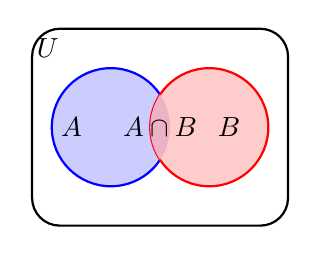
\begin{tikzpicture}[scale=0.5]
            \draw [rounded corners=10pt, thick] (-3,-2.5) rectangle (3.5,2.5);
            \node at (-2.6,2) {$U$};

            % Draw set A
            \draw [blue, thick, fill=blue!20] (-1,0) circle (1.5);
            \node at (-2,0) {$A$};

            % Draw set B
            \draw [red, thick, fill=red!20] (1.5,0) circle (1.5);
            \node at (2,0) {$B$};

            % Highlight A ∩ B
            \begin{scope}
                \clip (-1,0) circle (1.5);
                \fill[purple!30] (1.5,0) circle (1.5);
            \end{scope}
            \node at (0.25,0) {$A \cap B$};
        \end{tikzpicture}
        \captionof{figure}{定理韦恩图可视化}
    \end{minipage}
\end{theorem}

\begin{example}
    已知全集 $U=\{1,2,3,4,5,6,7\} \quad A=\{2,4,5,7\} \quad B=\{3,4,5\}$
    求 $(C_\cup A) \cup(C_\cup B)$ ．
\end{example}

\begin{solution}
    解：法一（常规法）：
    $$
        C_{\cup} A=\{1,3,6\} \quad C_{\cup} B=\{1,2,6,7\}
    $$
    则：$(C_{\cup} A) \cup(C_{\cup} B)=\{1,2,3,6,7\}$

    法二：根据德摩根定理可知：
    $\left(C_{\cup A}\right) \cup\left(C_{\cup B}\right)=C_{\cup}(A \cap B)$ ．
    $$
        A \cap B=\{4,5\} \quad C_v(A \cap B)=\{1,2,3,6,7\}
    $$
\end{solution}

\subsection{容斥原理}

\begin{definition}[容斥原理]
    对于两个集合 $A$ 和 $B$，它们的并集的元素个数可以通过以下公式计算：

    用记号：$\mathrm{card}(A)$来表示$A$中的元素个数（在此，我们简化为使用 $|A|$表示$A$中的元素个数），那么有：
    $$|A\cup B| = |A|+|B|-|A\cap B|$$
\end{definition}

\begin{proof}
    要证明上式，首先要说明：
    $$A\cap B=\emptyset \implies |A\cup B| = |A|+|B|$$
    和
    $$B\subset A \implies |A-B| = |A|-|B|$$

    对于有限集合，这两个式子是显然成立的，无限集合我们不做考虑。

    其次，要理解：
    $$A\cup B = (A-A\cap B) + (B-A\cap B) + A\cap B$$
    并且上式出现的三个集合$A-A\cap B$，$B-A\cap B$，$A\cap B$是互不相交的。

    最后就可以得到：
    \begin{align*}
          & |A\cup B|                                 \\
        = & |(A-A\cap B| + (B-A\cap B) + A\cap B)     \\
        = & |A-A\cap B| + |B-A\cap B| + |A\cap B|     \\
        = & |A|-|A\cap B| + |B|-|A\cap B| + |A\cap B| \\
        = & |A|+|B|-|A\cap B|
    \end{align*}
\end{proof}

\begin{example}
    某学校的一个年级共有100名学生，他们可以选择学习数学、物理、化学三门选修课。已知：
    \begin{itemize}
        \item 选修数学的学生有 50 人。选修物理的学生有 55 人。选修化学的学生有 60 人。
        \item 至少选修数学或物理一门的有 80 人。至少选修物理或化学一门的有 90 人。至少选修数学或化学一门的有 85 人。
        \item 每位学生至少选修了三门中的一门。
    \end{itemize}
    根据以上信息，求解以下问题：
    \begin{enumerate}
        \item 有多少学生同时选修了数学和物理？
        \item 有多少学生同时选修了数学、物理和化学三门课程？
    \end{enumerate}
\end{example}

\begin{solution}
    我们设集合 $A$ 为选修数学的学生集合，集合 $B$ 物理，集合 $C$ 为化学。
    根据题意，我们有：
    \begin{itemize}
        \item $|A| = 50$, $|B| = 55$, $|C| = 60$
        \item $|A \cup B| = 80$, $|B \cup C| = 90$, $|A \cup C| = 85$
        \item $|A \cup B \cup C| = 100$
    \end{itemize}

    \textbf{1. 求同时选修数学和物理的学生人数}

    这相当于求解集合 $A$ 和 $B$ 的交集大小，即 $|A \cap B|$。
    根据集合的容斥原理公式：
    $|A \cap B| = |A| + |B| - |A \cup B|$
    代入数据得：
    $|A \cap B| = 50 + 55 - 80 = 25$，所以，有 25 名学生同时选修了数学和物理。

    \textbf{2. 求同时选修三门课程的学生人数}

    这相当于求解集合 $A, B, C$ 的交集大小，即 $|A \cap B \cap C|$。
    而两两相交的集合大小已经在第一问解决：
    $$|A \cap B| = 25$$
    $$|B \cap C| = |B| + |C| - |B \cup C| = 55 + 60 - 90 = 25$$
    $$|A \cap C| = |A| + |C| - |A \cup C| = 50 + 60 - 85 = 25$$

    根据三集合的容斥原理公式：
    $$|A \cup B \cup C| = |A| + |B| + |C| - (|A \cap B| + |B \cap C| + |A \cap C|) + |A \cap B \cap C|$$
    代入数据得：
    $$100 = 50 + 55 + 60 - (25 + 25 + 25) + |A \cap B \cap C|$$
    $$|A \cap B \cap C| = 10$$
\end{solution}

\begin{example}
    某中学的学生积极参加体育锻炼，其中有 $96 \%$ 的学生喜欢足球或游泳， $60 \%$ 的学生喜欢足球， $82 \%$ 的学生喜欢游泳，则该中学既喜欢足球又喜欢游泳的学生数占该校学生总数的比例是 （\qquad）
    \begin{tasks}(4)
        \task $62 \%$
        \task $56 \%$
        \task $46 \%$
        \task $42 \%$
    \end{tasks}
\end{example}

\v{2em}

\begin{example}
    已知集合 $\mathrm{U}=\mathrm{A} \cup \mathrm{B}$ 中有 $m$ 个元素， $\left(\mathrm{C}_{\mathrm{U}} \mathrm{A}\right) \cup\left(\mathrm{C}_{\mathrm{U}} \mathrm{B}\right)$ 中有 $n$ 个元素。若 $\mathrm{A} \cap \mathrm{B}$ 非空，则 $A \cap B$ 的元素个数为 （\qquad）
    \begin{tasks}(4)
        \task $m n$
        \task $m+n$
        \task $n-m$
        \task $m-n$
    \end{tasks}
\end{example}

\begin{solution}
    此处应该选 D 项，根据容斥原理易得。
\end{solution}